\documentclass[a4paper,12pt]{article}
\usepackage[utf8]{inputenc}
\usepackage[cm,empty]{fullpage}
\usepackage[T2A]{fontenc}
\usepackage[english, russian]{babel}
\usepackage{amssymb,amsmath,amsxtra,amsthm}
\usepackage{proof}
\usepackage[pdftex]{graphicx}
\usepackage{wrapfig}
\usepackage{braket}
\usepackage{xcolor}

\usepackage[left=2cm,right=2cm,
    top=1cm,bottom=1cm,bindingoffset=0cm]{geometry}

\renewcommand{\leq}{\leqslant}
\renewcommand{\geq}{\geqslant}


\newcommand{\iiff}{\Longleftrightarrow}
\renewcommand{\iff}{\Leftrightarrow}
\newcommand{\nothing}{\varnothing}

\newtheorem*{rem}{Замечание}

\newcommand{\NN}{\mathbb{N}}
\newcommand{\ZZ}{\mathbb{Z}}
\newcommand{\Q}{\mathbb{Q}}
\newcommand{\A}{\mathbb{A}}
\newcommand{\R}{\mathbb{R}}
\renewcommand{\C}{\mathbb{C}}

\renewcommand{\phi}{\varphi}
\newcommand{\eps}{\varepsilon}

\newcounter{z}


\newcommand{\zs}{\refstepcounter{z}\vskip 10pt\par\noindent
\fbox{\textbf{12.\arabic{z}}} }

\newcommand{\z}{\refstepcounter{z}\vskip 20pt\noindent
\fbox{\textbf{\arabic{z}}} }

\renewcommand{\date}{{\bf 16 февраля 2021}} %Дата занятия

\newcommand{\dif}
{
------------------------------------------------------------------------------------------------------------------------------------------------------
}

\newcommand{\HSEhat}{
\vspace*{-0pt}
\noindent
\setcounter{z}{0}


{\bf \phantom{\date}  \large \hfill Математический анализ: \hfill \normalsize \date}

\vspace{5 pt}
{\bf \large \hfill  семинар 1\hfill }

\vspace{15 pt}
\centerline{ \large  Домашнее задание.}
\centerline{ \large  Кирилл Сетдеков}



\vspace*{10pt}
\setcounter{z}{0}

}

\begin{document}
\HSEhat


\subsection*{Задачи}

\begin{enumerate}

\item Найти предел
\begin{enumerate}
\item 
$
\lim\limits_{n\to \infty}\frac{(-2)^n + 3^n}{(-2)^{n+1} + 3^{n+1}}
$

\textbf{Решение:}\\
При $n\to \infty$, слагаемые с основанием 3 доминируют ответ.

$
\lim\limits_{n\to \infty}\frac{3^n}{3^{n+1}}=\lim\limits_{n\to \infty}(\frac{3}{3})^n\times\frac{1}{3}=\frac{1}{3}
$

\textbf{Ответ: $1/3$}


\item
$
\lim\limits_{n\to \infty}\frac{1 + a + \ldots + a^n}{1 + b + \ldots + b^n},\quad\text{где}\;|a|<1,\;|b|<1
$

\textbf{Решение:}\\
Числитель и знаменатель - сумма бесконечной убывающей геометрической прогрессии.

$
\lim\limits_{n\to \infty}\frac{\frac{1}{1-a}}{\frac{1}{1-b}}= \frac{1-b}{1-a}
$


\textbf{Ответ: $\frac{1-b}{1-a}$}


\end{enumerate}

\item Найти предел
\begin{enumerate}
\item 
$
\lim\limits_{x\to 1}\frac{x^2-1}{2x^2 - x - 1}
$

\textbf{Решение:}\\
Числитель и знаменатель дроби стремятся к 0. Используем правило Лопиталя.

$
\lim\limits_{x\to 1}\frac{x^2-1}{2x^2 - x - 1}=\lim\limits_{x\to 1}\frac{2x}{4x- 1} =2/3
$

\textbf{Ответ: $\frac{2}{3}$}


\item 
$
\lim\limits_{x\to 0}\frac{\ln(1 + x^2)}{\sin(\cos x - 1)}
$

\textbf{Решение:}\\
Числитель и знаменатель дроби стремятся к 0. Используем правило Лопиталя.

$
\lim\limits_{x\to 0}\frac{\ln(1 + x^2)}{\sin(\cos x - 1)}=\lim\limits_{x\to 0}\frac{\frac{2x}{1+x^2}}{\sin(x) (-\cos(\cos (x )-1 ))}=\lim\limits_{x\to 0}\frac{\frac{2(x^2 -1)}{(1+x^2)^2}}{\sin^2(x) (-\sin(\cos(x) -1 )) - \cos(x)( \cos(x) - 1)} = \frac{2}{-1}
$

\textbf{Ответ: $-2$}

\end{enumerate}


\item Найти производную
\begin{enumerate}
\item
$
y = \frac{1 + x - x^2}{1 - x + x^2}
$

\textbf{Решение:} \\
$y'(x) = \frac{(1-2x)\times(1 - x + x^2)+(1-2x)\times(1 + x - x^2)}{(1 - x + x^2)^2}=\frac{2-4x}{(1 - x + x^2)^2}$

\textbf{Ответ: $\frac{2-4x}{(1 - x + x^2)^2}$}

\item 
$
y = \ln(e^x + \sqrt{1 + e^{2x}})
$

\textbf{Решение:} \\
$$y'(x) = \frac{(e^x + \sqrt{1 + e^{2x}})'}{e^x + \sqrt{1 + e^{2x}}}=\frac{e^x + (\sqrt{1 + e^{2x}})'}{e^x + \sqrt{1 + e^{2x}}}=\frac{e^x + \frac{2e^{2x}}{2\sqrt{1 + e^{2x}}}}{e^x + \sqrt{1 + e^{2x}}}=\frac{e^{x} + \frac{e^{2x}}{\sqrt{1 + e^{2x}}}}{e^x + \sqrt{1 + e^{2x}}}=$$
$$=\frac{ \frac{e^{x}\sqrt{1 + e^{2x}}+e^{2x}}{\sqrt{1 + e^{2x}}}}{e^x + \sqrt{1 + e^{2x}}}=\frac{ \frac{e^{x}(\sqrt{1 + e^{2x}}+e^{x})}{\sqrt{1 + e^{2x}}}}{e^x + \sqrt{1 + e^{2x}}}=\frac{e^{x}}{\sqrt{1 + e^{2x}}}$$

\textbf{Ответ: $\frac{e^{x}}{\sqrt{1 + e^{2x}}}$}


\end{enumerate}

\item Найти $y'$, если
\begin{enumerate}
\item $y = f(\sin^2 x) + f(\cos^2 x)$

\textbf{Решение:} \\
$$y'(x) =f'(\sin^2 x)\times (2 \sin x \cos x)+ f'(\cos^2 x)\times (-2 \sin x \cos x)=$$
$$ =(f'(\sin^2 x)-f'(\cos^2 x))\times (2 \sin x \cos x)$$


\textbf{Ответ: $(f'(\sin^2 x)-f'(\cos^2 x))\times (2 \sin x \cos x)$}


\item $y = f(e^x) e^{f(x)}$

\textbf{Решение:} \\
$$y'(x) =f'(e^x) e^{f(x)}+f(e^x) (e^{f(x)})'= e^x f'(e^x) e^{f(x)}+f(e^x) e^{f(x)} f'(x) = $$
$$=e^{f(x)}(e^x f'(e^x)+f(e^x)f'(x))$$


\textbf{Ответ: $e^{f(x)}(e^x f'(e^x)+f(e^x)f'(x))$}

\end{enumerate}
где $f(x)$ -- дифференцируемая функция.


\item Исследовать на экстремумы
\begin{enumerate}
\item $y = (x+1)^{10}e^{-x}$


\textbf{Решение:} \\

$y' = 10(x+1)^{9}e^{-x} -(x+1)^{10}e^{-x}=e^{-x} ( 9-x) ( x+1)^9$

$y' = 0$ при $x = -1$ или $x = 9$

\centerline{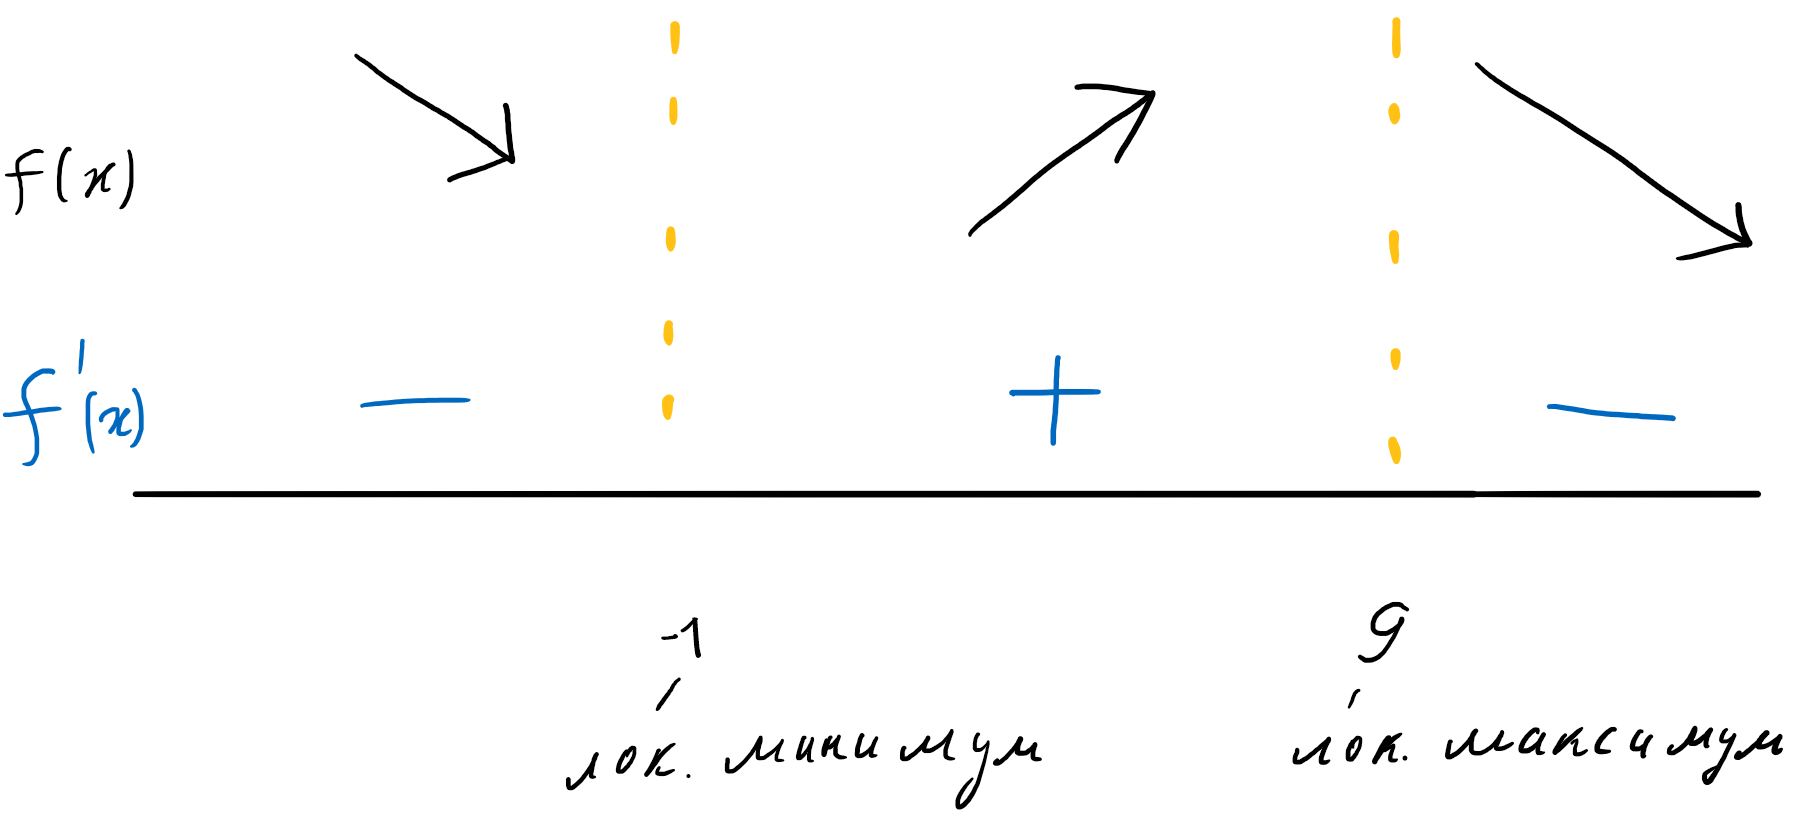
\includegraphics[width=\textwidth]{img/end2.png}}

-1 - локальный минимум, в 9 - локальный максимум.

\item $y = x + \frac{1}{x}$

\textbf{Решение:} \\
$y' = 1 - \frac{1}{x^2}$

$y \neq 0$ и $y' = 0$ при $x=\pm1$

\centerline{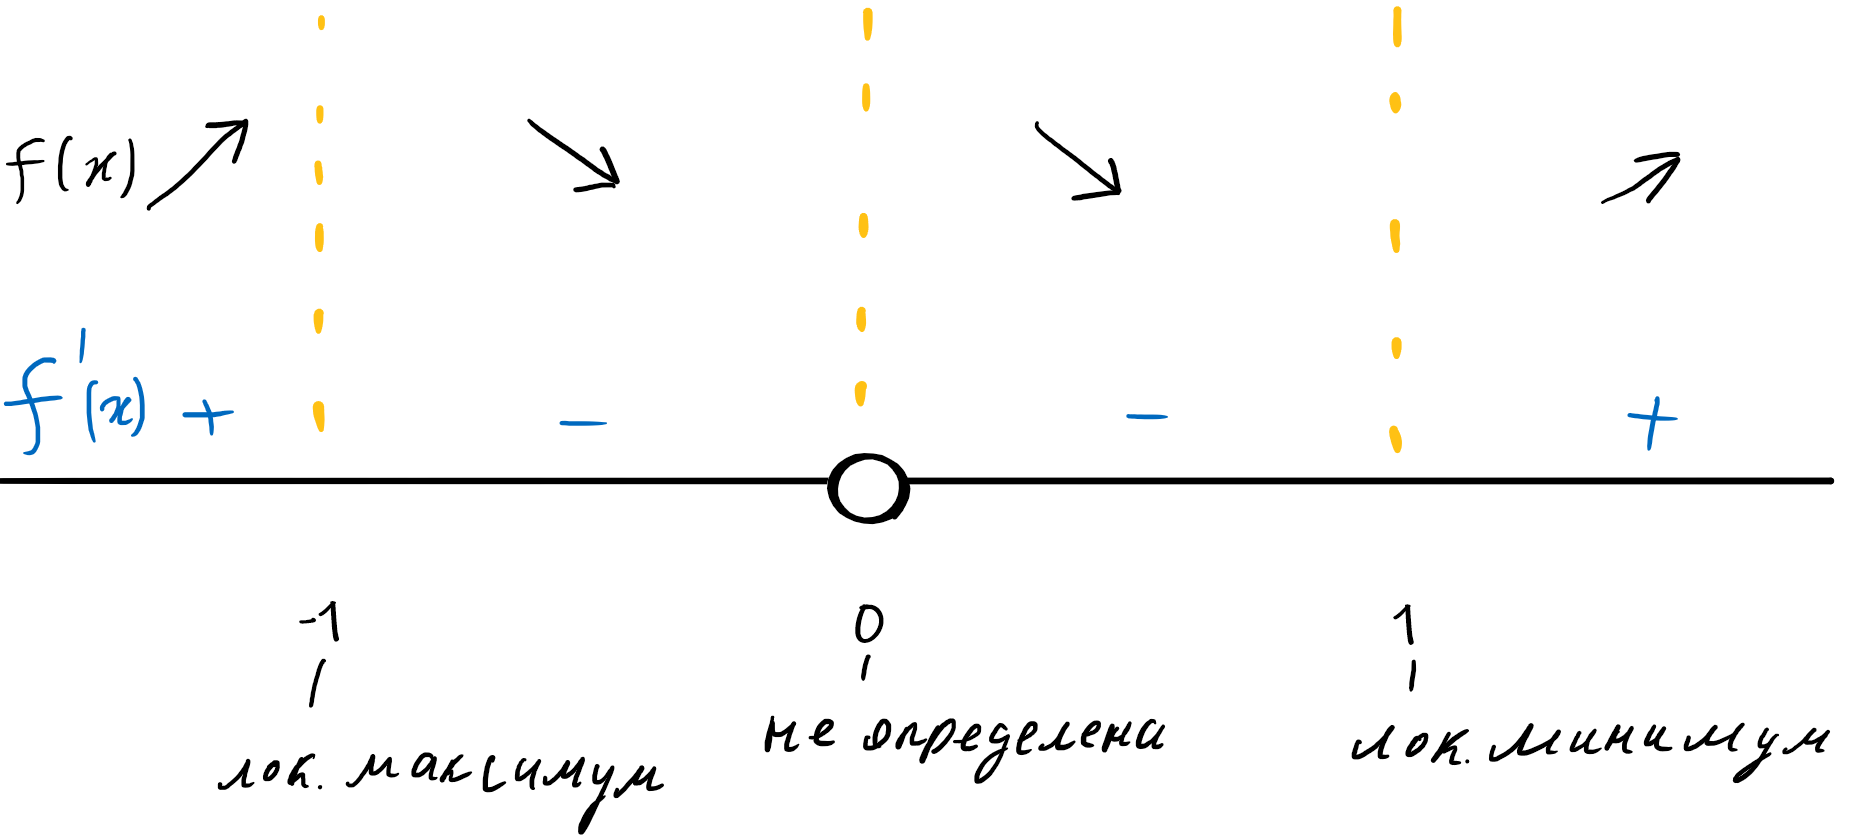
\includegraphics[width=\textwidth]{img/end1.png}}

-1 - локальный максимум, в 0 - функция не определена $
\lim\limits_{x\to +0}y = +\infty
$ и $
\lim\limits_{x\to -0}y = -\infty
$, в 1 - локальный минимум.

\end{enumerate}

\end{enumerate}
\end{document}